% Options for packages loaded elsewhere
\PassOptionsToPackage{unicode}{hyperref}
\PassOptionsToPackage{hyphens}{url}
\PassOptionsToPackage{dvipsnames,svgnames,x11names}{xcolor}
%
\documentclass[
  a4paper,
]{article}

\usepackage{amsmath,amssymb}
\usepackage{lmodern}
\usepackage{iftex}
\ifPDFTeX
  \usepackage[T1]{fontenc}
  \usepackage[utf8]{inputenc}
  \usepackage{textcomp} % provide euro and other symbols
\else % if luatex or xetex
  \usepackage{unicode-math}
  \defaultfontfeatures{Scale=MatchLowercase}
  \defaultfontfeatures[\rmfamily]{Ligatures=TeX,Scale=1}
\fi
% Use upquote if available, for straight quotes in verbatim environments
\IfFileExists{upquote.sty}{\usepackage{upquote}}{}
\IfFileExists{microtype.sty}{% use microtype if available
  \usepackage[]{microtype}
  \UseMicrotypeSet[protrusion]{basicmath} % disable protrusion for tt fonts
}{}
\makeatletter
\@ifundefined{KOMAClassName}{% if non-KOMA class
  \IfFileExists{parskip.sty}{%
    \usepackage{parskip}
  }{% else
    \setlength{\parindent}{0pt}
    \setlength{\parskip}{6pt plus 2pt minus 1pt}}
}{% if KOMA class
  \KOMAoptions{parskip=half}}
\makeatother
\usepackage{xcolor}
\usepackage[top=30mm,left=20mm,heightrounded]{geometry}
\setlength{\emergencystretch}{3em} % prevent overfull lines
\setcounter{secnumdepth}{5}
% Make \paragraph and \subparagraph free-standing
\ifx\paragraph\undefined\else
  \let\oldparagraph\paragraph
  \renewcommand{\paragraph}[1]{\oldparagraph{#1}\mbox{}}
\fi
\ifx\subparagraph\undefined\else
  \let\oldsubparagraph\subparagraph
  \renewcommand{\subparagraph}[1]{\oldsubparagraph{#1}\mbox{}}
\fi

\usepackage{color}
\usepackage{fancyvrb}
\newcommand{\VerbBar}{|}
\newcommand{\VERB}{\Verb[commandchars=\\\{\}]}
\DefineVerbatimEnvironment{Highlighting}{Verbatim}{commandchars=\\\{\}}
% Add ',fontsize=\small' for more characters per line
\usepackage{framed}
\definecolor{shadecolor}{RGB}{241,243,245}
\newenvironment{Shaded}{\begin{snugshade}}{\end{snugshade}}
\newcommand{\AlertTok}[1]{\textcolor[rgb]{0.68,0.00,0.00}{#1}}
\newcommand{\AnnotationTok}[1]{\textcolor[rgb]{0.37,0.37,0.37}{#1}}
\newcommand{\AttributeTok}[1]{\textcolor[rgb]{0.40,0.45,0.13}{#1}}
\newcommand{\BaseNTok}[1]{\textcolor[rgb]{0.68,0.00,0.00}{#1}}
\newcommand{\BuiltInTok}[1]{\textcolor[rgb]{0.00,0.23,0.31}{#1}}
\newcommand{\CharTok}[1]{\textcolor[rgb]{0.13,0.47,0.30}{#1}}
\newcommand{\CommentTok}[1]{\textcolor[rgb]{0.37,0.37,0.37}{#1}}
\newcommand{\CommentVarTok}[1]{\textcolor[rgb]{0.37,0.37,0.37}{\textit{#1}}}
\newcommand{\ConstantTok}[1]{\textcolor[rgb]{0.56,0.35,0.01}{#1}}
\newcommand{\ControlFlowTok}[1]{\textcolor[rgb]{0.00,0.23,0.31}{#1}}
\newcommand{\DataTypeTok}[1]{\textcolor[rgb]{0.68,0.00,0.00}{#1}}
\newcommand{\DecValTok}[1]{\textcolor[rgb]{0.68,0.00,0.00}{#1}}
\newcommand{\DocumentationTok}[1]{\textcolor[rgb]{0.37,0.37,0.37}{\textit{#1}}}
\newcommand{\ErrorTok}[1]{\textcolor[rgb]{0.68,0.00,0.00}{#1}}
\newcommand{\ExtensionTok}[1]{\textcolor[rgb]{0.00,0.23,0.31}{#1}}
\newcommand{\FloatTok}[1]{\textcolor[rgb]{0.68,0.00,0.00}{#1}}
\newcommand{\FunctionTok}[1]{\textcolor[rgb]{0.28,0.35,0.67}{#1}}
\newcommand{\ImportTok}[1]{\textcolor[rgb]{0.00,0.46,0.62}{#1}}
\newcommand{\InformationTok}[1]{\textcolor[rgb]{0.37,0.37,0.37}{#1}}
\newcommand{\KeywordTok}[1]{\textcolor[rgb]{0.00,0.23,0.31}{#1}}
\newcommand{\NormalTok}[1]{\textcolor[rgb]{0.00,0.23,0.31}{#1}}
\newcommand{\OperatorTok}[1]{\textcolor[rgb]{0.37,0.37,0.37}{#1}}
\newcommand{\OtherTok}[1]{\textcolor[rgb]{0.00,0.23,0.31}{#1}}
\newcommand{\PreprocessorTok}[1]{\textcolor[rgb]{0.68,0.00,0.00}{#1}}
\newcommand{\RegionMarkerTok}[1]{\textcolor[rgb]{0.00,0.23,0.31}{#1}}
\newcommand{\SpecialCharTok}[1]{\textcolor[rgb]{0.37,0.37,0.37}{#1}}
\newcommand{\SpecialStringTok}[1]{\textcolor[rgb]{0.13,0.47,0.30}{#1}}
\newcommand{\StringTok}[1]{\textcolor[rgb]{0.13,0.47,0.30}{#1}}
\newcommand{\VariableTok}[1]{\textcolor[rgb]{0.07,0.07,0.07}{#1}}
\newcommand{\VerbatimStringTok}[1]{\textcolor[rgb]{0.13,0.47,0.30}{#1}}
\newcommand{\WarningTok}[1]{\textcolor[rgb]{0.37,0.37,0.37}{\textit{#1}}}

\providecommand{\tightlist}{%
  \setlength{\itemsep}{0pt}\setlength{\parskip}{0pt}}\usepackage{longtable,booktabs,array}
\usepackage{calc} % for calculating minipage widths
% Correct order of tables after \paragraph or \subparagraph
\usepackage{etoolbox}
\makeatletter
\patchcmd\longtable{\par}{\if@noskipsec\mbox{}\fi\par}{}{}
\makeatother
% Allow footnotes in longtable head/foot
\IfFileExists{footnotehyper.sty}{\usepackage{footnotehyper}}{\usepackage{footnote}}
\makesavenoteenv{longtable}
\usepackage{graphicx}
\makeatletter
\def\maxwidth{\ifdim\Gin@nat@width>\linewidth\linewidth\else\Gin@nat@width\fi}
\def\maxheight{\ifdim\Gin@nat@height>\textheight\textheight\else\Gin@nat@height\fi}
\makeatother
% Scale images if necessary, so that they will not overflow the page
% margins by default, and it is still possible to overwrite the defaults
% using explicit options in \includegraphics[width, height, ...]{}
\setkeys{Gin}{width=\maxwidth,height=\maxheight,keepaspectratio}
% Set default figure placement to htbp
\makeatletter
\def\fps@figure{htbp}
\makeatother
\newlength{\cslhangindent}
\setlength{\cslhangindent}{1.5em}
\newlength{\csllabelwidth}
\setlength{\csllabelwidth}{3em}
\newlength{\cslentryspacingunit} % times entry-spacing
\setlength{\cslentryspacingunit}{\parskip}
\newenvironment{CSLReferences}[2] % #1 hanging-ident, #2 entry spacing
 {% don't indent paragraphs
  \setlength{\parindent}{0pt}
  % turn on hanging indent if param 1 is 1
  \ifodd #1
  \let\oldpar\par
  \def\par{\hangindent=\cslhangindent\oldpar}
  \fi
  % set entry spacing
  \setlength{\parskip}{#2\cslentryspacingunit}
 }%
 {}
\usepackage{calc}
\newcommand{\CSLBlock}[1]{#1\hfill\break}
\newcommand{\CSLLeftMargin}[1]{\parbox[t]{\csllabelwidth}{#1}}
\newcommand{\CSLRightInline}[1]{\parbox[t]{\linewidth - \csllabelwidth}{#1}\break}
\newcommand{\CSLIndent}[1]{\hspace{\cslhangindent}#1}

\makeatletter
\makeatother
\makeatletter
\makeatother
\makeatletter
\@ifpackageloaded{caption}{}{\usepackage{caption}}
\AtBeginDocument{%
\ifdefined\contentsname
  \renewcommand*\contentsname{Table of contents}
\else
  \newcommand\contentsname{Table of contents}
\fi
\ifdefined\listfigurename
  \renewcommand*\listfigurename{List of Figures}
\else
  \newcommand\listfigurename{List of Figures}
\fi
\ifdefined\listtablename
  \renewcommand*\listtablename{List of Tables}
\else
  \newcommand\listtablename{List of Tables}
\fi
\ifdefined\figurename
  \renewcommand*\figurename{Figure}
\else
  \newcommand\figurename{Figure}
\fi
\ifdefined\tablename
  \renewcommand*\tablename{Table}
\else
  \newcommand\tablename{Table}
\fi
}
\@ifpackageloaded{float}{}{\usepackage{float}}
\floatstyle{ruled}
\@ifundefined{c@chapter}{\newfloat{codelisting}{h}{lop}}{\newfloat{codelisting}{h}{lop}[chapter]}
\floatname{codelisting}{Listing}
\newcommand*\listoflistings{\listof{codelisting}{List of Listings}}
\makeatother
\makeatletter
\@ifpackageloaded{caption}{}{\usepackage{caption}}
\@ifpackageloaded{subcaption}{}{\usepackage{subcaption}}
\makeatother
\makeatletter
\@ifpackageloaded{tcolorbox}{}{\usepackage[many]{tcolorbox}}
\makeatother
\makeatletter
\@ifundefined{shadecolor}{\definecolor{shadecolor}{rgb}{.97, .97, .97}}
\makeatother
\makeatletter
\makeatother
\ifLuaTeX
  \usepackage{selnolig}  % disable illegal ligatures
\fi
\IfFileExists{bookmark.sty}{\usepackage{bookmark}}{\usepackage{hyperref}}
\IfFileExists{xurl.sty}{\usepackage{xurl}}{} % add URL line breaks if available
\urlstyle{same} % disable monospaced font for URLs
\hypersetup{
  pdftitle={inlabru : Convenient fitting of Bayesian digital soil mapping models using INLA-SPDE},
  pdfauthor={Nicolas Saby1; Thomas Opitz2},
  colorlinks=true,
  linkcolor={blue},
  filecolor={Maroon},
  citecolor={Blue},
  urlcolor={Blue},
  pdfcreator={LaTeX via pandoc}}

\title{inlabru : Convenient fitting of Bayesian digital soil mapping
models using INLA-SPDE}
\author{Nicolas Saby\textsuperscript{1} \and Thomas
Opitz\textsuperscript{2}}
\date{4/24/23}

\begin{document}
\maketitle
\ifdefined\Shaded\renewenvironment{Shaded}{\begin{tcolorbox}[frame hidden, enhanced, interior hidden, borderline west={3pt}{0pt}{shadecolor}, sharp corners, breakable, boxrule=0pt]}{\end{tcolorbox}}\fi

\renewcommand*\contentsname{Table of contents}
{
\hypersetup{linkcolor=}
\setcounter{tocdepth}{3}
\tableofcontents
}
\textsuperscript{1} INRAE, Info\&Sols, Orléans, France\\
\textsuperscript{2} INRAE, BioSP, Avignon, France

\hypertarget{introduction}{%
\section{Introduction}\label{introduction}}

Pedometricians are nowadays heavy users of Machine Learning (ML)
approaches with on the top the widely used random forest algorithm, see
for example (L. Poggio et al. 2021). These algorithms are indeed
particularly well adapted to the management of large data sets to map
soil properties on large geographic areas in a wide range of situations.
The techniques are based on classification and regression algorithms,
but they take no account of spatial correlations in residuals (Heuvelink
and Webster 2022). This trend towards heavy use of ML tools also seems
to be accompanied by a diminished use of geostatistical techniques that
often require more computer resources but also profound statistical
skills to construct and fine-tune models. Often, prediction is performed
in several steps (\emph{eg} regression or any other machine learning
prediction in step 1, followed by spatial kriging of the residuals in
step 2), but then an accurate assessment of the prediction uncertainties
is difficult since uncertainties from the first step must be propagated
through to the second step.

In this paper, we propose to solve these issues by using the fully
Bayesian estimation framework based on the integrated nested Laplace
approximation (INLA,(Rue, Martino, and Chopin 2009)), combined with the
so-called stochastic partial differential equation approach (SPDE,
Lindgren, Rue, and Lindström 2011) providing numerically convenient
representations of Gaussian processes over continuous space. Over the
last decade, the INLA method has become the most popular tool in spatial
statistics for estimating a wide variety of Generalized Additive Mixed
Models (i.e., Generalized Additive Models with random effects) in a
Bayesian setting. It is a relatively easy-to-use alternative to
traditional Markov chain Monte Carlo methods by providing off-the-shelf
implementation of fast and accurate deterministic approximations of
posterior inferences for a large class of models. INLA with SPDE is a
powerful combination to handle very large spatial data sets. Models are
formulated as Bayesian hierarchical models where covariate effects and
Gaussian processes can be additively included in a latent process (that
is not directly), whereas the probability distribution of observations
can be of various nature (continuous such as gaussian, skew-gaussian,
gamma, extreme-value, or discrete such as Poisson, binomial, negative
binomial) and its parameters are controlled by the latent process.

INLA-SPDE was already introduced by (Laura Poggio et al. 2016) or (Huang
2017) to the pedometrics community. However, wider use of this approach
by the community was probably hindered by the complexity of the INLA R
package. Recently, the \texttt{inlabru} R package (Yuan et al. 2017),
originally developed with a strong focus on point process models for
discrete data in ecology, has integrated a range of functions to help in
implementing INLA-SPDE models in a more convenient way through a more
ergonomic interface. We propose here to illustrate how this package
works by using a simple and classical regression kriging approach as an
example.

\hypertarget{set-up}{%
\section{Set up}\label{set-up}}

\hypertarget{load-packages}{%
\subsection{Load packages}\label{load-packages}}

We use here the set of R packages given in the list below.

The latest version of R (eg \textgreater4.2) should be installed on your
computer for using the \texttt{inlabru} package. The classical dataset
for the Meuse area that we use here is available in the
\texttt{gstat}package.

\begin{Shaded}
\begin{Highlighting}[]
\FunctionTok{library}\NormalTok{(INLA)}
\FunctionTok{library}\NormalTok{(inlabru)}
\FunctionTok{library}\NormalTok{(dplyr)}
\FunctionTok{library}\NormalTok{(tmap)}
\FunctionTok{library}\NormalTok{(gstat) }\CommentTok{\# for the meuse data}
\FunctionTok{library}\NormalTok{(tmap)}
\FunctionTok{library}\NormalTok{(ggplot2)}
\end{Highlighting}
\end{Shaded}

The \texttt{inlabru} method is a convenient wrapper for the
\texttt{INLA::inla} function and provides multiple enhancements, such as
an improved integration of spatial object classes of type \texttt{sp} in
R, more convenient syntax for defining the structure of the model,
convenient functions to perform Bayesian prediction using simulations
from the estimated posterior model, and estimation facilities for
certain model structures that are not possible with the classical
\texttt{INLA} package.

\hypertarget{point-data-and-rasters}{%
\subsection{Point data and rasters}\label{point-data-and-rasters}}

We use the open data \texttt{meuse} from the \texttt{gstat} package

\begin{Shaded}
\begin{Highlighting}[]
\FunctionTok{data}\NormalTok{(meuse)}
\FunctionTok{data}\NormalTok{(meuse.grid)}

\FunctionTok{str}\NormalTok{(meuse)}
\end{Highlighting}
\end{Shaded}

\begin{verbatim}
'data.frame':   155 obs. of  14 variables:
 $ x      : num  181072 181025 181165 181298 181307 ...
 $ y      : num  333611 333558 333537 333484 333330 ...
 $ cadmium: num  11.7 8.6 6.5 2.6 2.8 3 3.2 2.8 2.4 1.6 ...
 $ copper : num  85 81 68 81 48 61 31 29 37 24 ...
 $ lead   : num  299 277 199 116 117 137 132 150 133 80 ...
 $ zinc   : num  1022 1141 640 257 269 ...
 $ elev   : num  7.91 6.98 7.8 7.66 7.48 ...
 $ dist   : num  0.00136 0.01222 0.10303 0.19009 0.27709 ...
 $ om     : num  13.6 14 13 8 8.7 7.8 9.2 9.5 10.6 6.3 ...
 $ ffreq  : Factor w/ 3 levels "1","2","3": 1 1 1 1 1 1 1 1 1 1 ...
 $ soil   : Factor w/ 3 levels "1","2","3": 1 1 1 2 2 2 2 1 1 2 ...
 $ lime   : Factor w/ 2 levels "0","1": 2 2 2 1 1 1 1 1 1 1 ...
 $ landuse: Factor w/ 15 levels "Aa","Ab","Ag",..: 4 4 4 11 4 11 4 2 2 15 ...
 $ dist.m : num  50 30 150 270 380 470 240 120 240 420 ...
\end{verbatim}

\begin{Shaded}
\begin{Highlighting}[]
\FunctionTok{str}\NormalTok{(meuse.grid)}
\end{Highlighting}
\end{Shaded}

\begin{verbatim}
'data.frame':   3103 obs. of  7 variables:
 $ x     : num  181180 181140 181180 181220 181100 ...
 $ y     : num  333740 333700 333700 333700 333660 ...
 $ part.a: num  1 1 1 1 1 1 1 1 1 1 ...
 $ part.b: num  0 0 0 0 0 0 0 0 0 0 ...
 $ dist  : num  0 0 0.0122 0.0435 0 ...
 $ soil  : Factor w/ 3 levels "1","2","3": 1 1 1 1 1 1 1 1 1 1 ...
 $ ffreq : Factor w/ 3 levels "1","2","3": 1 1 1 1 1 1 1 1 1 1 ...
\end{verbatim}

The first action is to create \texttt{sp} objects:

\begin{itemize}
\item
  a \texttt{SpatialPointsDataFrame} corresponding to the regression
  matrix and,
\item
  the prediction grid, here already provided in the
  \texttt{meuse.grid}-object along with covariates.
\end{itemize}

\begin{Shaded}
\begin{Highlighting}[]
\FunctionTok{coordinates}\NormalTok{(meuse) }\OtherTok{\textless{}{-}} \FunctionTok{c}\NormalTok{(}\StringTok{\textquotesingle{}x\textquotesingle{}}\NormalTok{,}\StringTok{\textquotesingle{}y\textquotesingle{}}\NormalTok{)}

\FunctionTok{coordinates}\NormalTok{(meuse.grid) }\OtherTok{\textless{}{-}} \FunctionTok{c}\NormalTok{(}\StringTok{"x"}\NormalTok{,}\StringTok{"y"}\NormalTok{)}
\FunctionTok{gridded}\NormalTok{(meuse.grid) }\OtherTok{=} \ConstantTok{TRUE}
\end{Highlighting}
\end{Shaded}

\hypertarget{fully-bayesian-dsm-approach}{%
\section{Fully Bayesian DSM
approach}\label{fully-bayesian-dsm-approach}}

\hypertarget{the-hierarchical-dsm-model}{%
\subsection{The hierarchical DSM
model}\label{the-hierarchical-dsm-model}}

We construct a hierarchical model for the soil property \(z(s)\) of a
spatial location \(s\) in the framework of the prediction in the
presence of exhaustive ancillary information. We will assume the
following linkage between model components and observations, where we
denote the latent process by \(\eta(s)\). In this paper, \(z\) will
correspond to the organic matter, \texttt{om}.

\[
\eta(s) \sim {\text{Intercept}} + \underbrace{ \sum_{i\in \text{scorpan}}\beta_i z_i(s)}_{\text{Covariates} } +\underbrace{W(s)}_{\text{Spatial Gaussian field}}
\] The spatial field \(W(s)\) captures autocorrelation not explained by
the covariates. The latent process \(\eta(s)\) will then be used in the
observation-likelihood, which is here chosen as gamma distribution as
soil carbon is known to present a heavy-tailed distribution.

We use the \texttt{\textbar{}} notation to indicate conditioning of the
property at the left side of \texttt{\textbar{}} o the parameters given
to the right side of \texttt{\textbar{}}. This leads to the following
hierarchical formulation for the observations,

\[
z(s) | (\eta(s),\theta) \sim \Gamma(\exp(\eta(s_i)), \tau),
\] where the Gamma distribution is parametrized in a way such that
\(\exp(\eta(s_i))\) is its mean and \(\tau\) is a dispersion parameter
related to the variance around the mean.
\(\theta = (\theta_\eta, \tau)\) with \(\theta_\eta\) the
hyperparameters controlling the linear predictors \(\eta\).

Moreover different observations \(z(s)\) are conditionally independent
given the latent process \(\eta(s)\) and the hyperparameters in
\(\theta\) controlling it. This means that we include a
\texttt{nugget\ effect} or \texttt{measurement\ error} with variance
\(\sigma^2\) in the model.

\hypertarget{construction-of-the-mesh-for-the-spde-model}{%
\subsection{Construction of the mesh for the SPDE
model}\label{construction-of-the-mesh-for-the-spde-model}}

\texttt{INLA} and \texttt{inlabru} use a space triangulation method to
estimate spatial Gaussian effects with a Matérn covariance function. The
latent spatial Gaussian random field is computed at the mesh nodes by
resolving a Stochastic Partial Differential Equation (SPDE), while it is
computed elsewhere by linear interpolation between the mesh nodes. The
mesh definition is based on a trade-off between the finer spatial scale
of the spatial effect (higher resolution) and a lower number of nodes
(lower resolution), where having less nodes usually comes with faster
calculations. Many applications already come with a regular grid used to
discretize space, such as the \texttt{meuse.grid} object here, but often
it still makes sense to choose different nodes for the space
triangulation used to represent the Gaussian field \(W(s)\), especially
in cases where the resolution of the grid from the data is too high for
being handled directly by INLA. Below, we present how to build a mesh
where the construction of the mesh nodes is initialized using the set of
coordinates of the calibration sites. This makes sense since can be
useful to have a mesh that is relatively denser in areas with many
calibration sites (where data provide more information).

First, we create a matrix \texttt{xyMesh} with coordinates of the sites.
Next, we define the boundaries of the domain used for computing the
spatial latent effect with the SPDE approach. Generally, it is better to
compute an internal boundary (delimiting the study area where we want to
predict) and an external boundary (providing an extension zone around
the study area that is necessary to avoid strong boundary effects from
the SPDE) with different resolutions. The purpose of the extension zone
is to push the outer boundary away from the study area, and we can set a
lower mesh resolution in this extension zone where we do not want to
predict the soil property.

The \texttt{INLA::inla.mesh.2d} function creates a triangle mesh based
on initial point locations, specified or automatic boundaries, and mesh
quality parameters, in particular the \texttt{cutoff}. This tuning
parameter sets the minimum length of edges between two nodes and allows
to keep the number of nodes at most moderately high and to avoid
instabilities in computations related to the covariance structure due to
very high Gaussian correlation at nodes that are very close in space.
More information is provided here: https://rpubs.com/jafet089/886687

\begin{Shaded}
\begin{Highlighting}[]
\NormalTok{cutoffValue }\OtherTok{=} \DecValTok{50} \CommentTok{\# in meter}

\NormalTok{xyMesh }\OtherTok{\textless{}{-}} \FunctionTok{rbind}\NormalTok{(}\FunctionTok{coordinates}\NormalTok{(meuse)) }\CommentTok{\# transform into matrix}

\NormalTok{max.edge }\OtherTok{=} \FunctionTok{diff}\NormalTok{(}\FunctionTok{range}\NormalTok{(xyMesh[,}\DecValTok{1}\NormalTok{]))}\SpecialCharTok{/}\NormalTok{(}\DecValTok{3}\SpecialCharTok{*}\DecValTok{5}\NormalTok{)}
\NormalTok{bound.outer }\OtherTok{=} \FunctionTok{diff}\NormalTok{(}\FunctionTok{range}\NormalTok{(}\FunctionTok{range}\NormalTok{(xyMesh[,}\DecValTok{1}\NormalTok{])))}\SpecialCharTok{/}\DecValTok{3}

\NormalTok{bndint }\OtherTok{\textless{}{-}} \FunctionTok{inla.nonconvex.hull}\NormalTok{(meuse, }\AttributeTok{convex=}\SpecialCharTok{{-}}\NormalTok{.}\DecValTok{05}\NormalTok{)}
\NormalTok{bndext }\OtherTok{\textless{}{-}} \FunctionTok{inla.nonconvex.hull}\NormalTok{(meuse, }\AttributeTok{convex=}\SpecialCharTok{{-}}\NormalTok{.}\DecValTok{3}\NormalTok{)}

\CommentTok{\# Use of inla.mesh.2d }
\NormalTok{mesh }\OtherTok{=} \FunctionTok{inla.mesh.2d}\NormalTok{(}\AttributeTok{loc=}\NormalTok{xyMesh,}
                    \AttributeTok{boundary =} \FunctionTok{list}\NormalTok{(}\AttributeTok{int =}\NormalTok{ bndint,}
                                    \AttributeTok{out =}\NormalTok{ bndext),}
                    \AttributeTok{max.edge =} \FunctionTok{c}\NormalTok{(}\DecValTok{1}\NormalTok{,}\DecValTok{3}\NormalTok{)}\SpecialCharTok{*}\NormalTok{max.edge, }
                    \AttributeTok{cutoff =}\NormalTok{ cutoffValue,}
                    \AttributeTok{crs =}\NormalTok{ meuse}\SpecialCharTok{@}\NormalTok{proj4string}\SpecialCharTok{@}\NormalTok{projargs)}
\FunctionTok{ggplot}\NormalTok{() }\SpecialCharTok{+}
  \FunctionTok{gg}\NormalTok{(mesh) }\SpecialCharTok{+}
  \FunctionTok{gg}\NormalTok{(meuse) }\SpecialCharTok{+}
  \FunctionTok{coord\_equal}\NormalTok{()}
\end{Highlighting}
\end{Shaded}

\begin{figure}[H]

{\centering 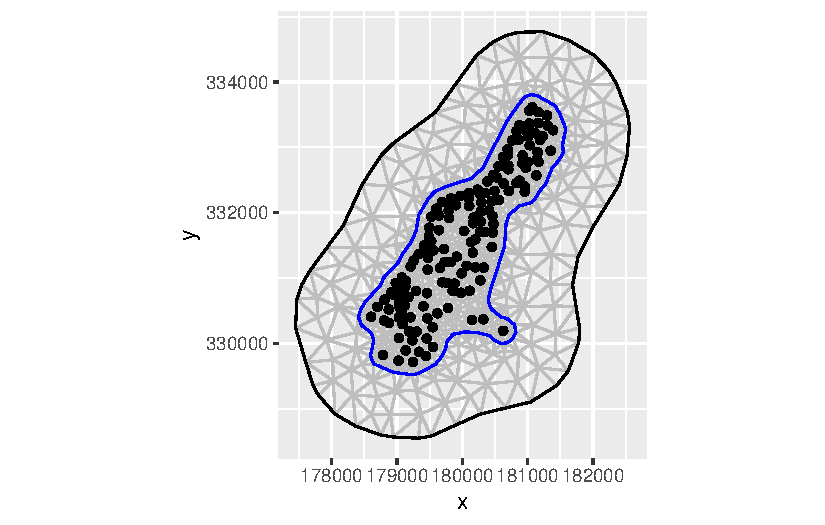
\includegraphics{pedometron_files/figure-pdf/unnamed-chunk-4-1.pdf}

}

\end{figure}

\hypertarget{defining-the-spatial-gaussian-random-field-ws}{%
\subsection{\texorpdfstring{Defining the spatial Gaussian random field
\(W(s)\)}{Defining the spatial Gaussian random field W(s)}}\label{defining-the-spatial-gaussian-random-field-ws}}

We choose the Matérn covariance function for the Gaussian random field
because it can be easily used within \texttt{INLA} through the SPDE
approach providing convenient numerical representations for estimation
with large numbers of observations and mesh nodes. The Matérn covariance
in \texttt{INLA} depends on three parameters: - a fractional order
parameter *alpha* in the SPDE linked to the smoothness of the solution
(which has to be fixed by the user), - a standard deviation parameter
*sigma* and, - a spatial correlation parameter known as the *range*.

We specify these parameters in our model by selecting a penalized
complexity prior using the \texttt{INLA::inla.spde2.pcmatern} function.
For more details, please refer to the introduction to spatial models
with \texttt{INLA} in chapter 7 at
\textless https://becarioprecario.bitbucket.io/inla-gitbook/ch-spatial.html\textgreater.

\begin{Shaded}
\begin{Highlighting}[]
\NormalTok{matern }\OtherTok{\textless{}{-}}
\NormalTok{  INLA}\SpecialCharTok{::}\FunctionTok{inla.spde2.pcmatern}\NormalTok{(mesh,}
                      \AttributeTok{alpha =} \DecValTok{2}\NormalTok{,}
                      \AttributeTok{prior.sigma =} \FunctionTok{c}\NormalTok{(}\DecValTok{1}\NormalTok{, }\FloatTok{0.5}\NormalTok{),}\CommentTok{\# P(sigma \textgreater{} 1) = 0.5}
                      \AttributeTok{prior.range =} \FunctionTok{c}\NormalTok{(}\DecValTok{10000}\NormalTok{, }\FloatTok{0.9}\NormalTok{)  }\CommentTok{\# P(range \textless{} 10000 m) = 0.9}
\NormalTok{  )}
\end{Highlighting}
\end{Shaded}

\hypertarget{specify-the-hierarchical-model}{%
\subsection{Specify the hierarchical
model}\label{specify-the-hierarchical-model}}

We then specify the model components in the \texttt{cmp} object using
the convenient \texttt{inlabru} approach. We use as example the
following latent effects: an intercept, a linear relationship with the
covariate as fixed effect corresponding to the distance to the river,
and the Gaussian random field as random effect.

\begin{Shaded}
\begin{Highlighting}[]
\NormalTok{cmp }\OtherTok{\textless{}{-}}\NormalTok{ om }\SpecialCharTok{\textasciitilde{}} 
  \FunctionTok{field}\NormalTok{(coordinates, }\AttributeTok{model =}\NormalTok{ matern) }\SpecialCharTok{+} 
  \FunctionTok{Intercept}\NormalTok{(}\DecValTok{1}\NormalTok{) }\SpecialCharTok{+} 
  \FunctionTok{dist}\NormalTok{(dist, }\AttributeTok{model =} \StringTok{\textquotesingle{}linear\textquotesingle{}}\NormalTok{ )     }
\end{Highlighting}
\end{Shaded}

Finally, we fit the hierarchical model to the data using the
\texttt{bru} function of the \texttt{inlabru} package. This function
requires the model components defined earlier (\texttt{cmp}), the
dataset (\texttt{meuse}), the mesh (\texttt{mesh}) where the model will
be evaluated, and several options to control the INLA algorithm.

For handling the uncertainty stemming from the prior distributions of
hyperparameters (here the standard deviation and the correlation range),
we use the \texttt{eb} strategy as it is much quicker to compute but a
bit less accurate. This \texttt{empirical\ Bayes} approach sets the
hyperparameters to their \texttt{maximum\ a\ posteriori} for some of the
calculations performed during the estimation algorithm, that is, it uses
a mechanism similar to frequentist inference techniques for handling the
hyperparameters.

One need to indicate the likelihood family such as \texttt{gaussian},
\texttt{poisson} or \texttt{binomial}. By default family is
\texttt{gaussian}. A list of possible alternatives can be seen by typing
\texttt{names(inla.models()\$likelihood)}. It is therefore possible to
fit a wide range of model allowing to approach a great diversity of
problems in soil science. We use here the \texttt{gamma} family to cope
with heavy tail.

\begin{Shaded}
\begin{Highlighting}[]
\NormalTok{fit }\OtherTok{\textless{}{-}}\NormalTok{ inlabru}\SpecialCharTok{::}\FunctionTok{bru}\NormalTok{(}
  \AttributeTok{components =}\NormalTok{ cmp,}
  \AttributeTok{data =}\NormalTok{ meuse,}
  \AttributeTok{family =} \StringTok{"gamma"}\NormalTok{,}
  \AttributeTok{domain =} \FunctionTok{list}\NormalTok{(}\AttributeTok{coordinates =}\NormalTok{ mesh),}
  \AttributeTok{options =} \FunctionTok{list}\NormalTok{(}
    \AttributeTok{control.inla =} \FunctionTok{list}\NormalTok{(}\AttributeTok{int.strategy =} \StringTok{"eb"}\NormalTok{),}
    \AttributeTok{verbose =} \ConstantTok{FALSE}
\NormalTok{  )}
\NormalTok{)}
\end{Highlighting}
\end{Shaded}

The summary of the fitted model gives the posterior estimates of fixed
effects (intercept and elevation) and hyperparameters (standard
deviation and range of the Gaussian random field).

We can look at some summaries of the posterior distributions for the
parameters, for example the fixed effects (i.e.~the intercept) and the
hyper-parameters (i.e.~variance of the gaussian likelihood, the
precision of the RW1, and the parameters of the spatial field):

\begin{Shaded}
\begin{Highlighting}[]
\FunctionTok{summary}\NormalTok{(fit)}
\end{Highlighting}
\end{Shaded}

\begin{verbatim}
inlabru version: 2.7.0
INLA version: 22.12.16
Components:
field: main = spde(coordinates)
Intercept: main = linear(1)
dist: main = linear(dist)
Likelihoods:
  Family: 'gamma'
    Data class: 'SpatialPointsDataFrame'
    Predictor: om ~ .
Time used:
    Pre = 1.25, Running = 1.18, Post = 0.058, Total = 2.49 
Fixed effects:
            mean    sd 0.025quant 0.5quant 0.975quant   mode kld
Intercept  2.349 0.223      1.912    2.349      2.785  2.349   0
dist      -1.311 0.390     -2.076   -1.311     -0.547 -1.311   0

Random effects:
  Name    Model
    field SPDE2 model

Model hyperparameters:
                                                   mean      sd 0.025quant
Precision parameter for the Gamma observations   14.227   2.487      9.969
Range for field                                1760.208 831.851    781.670
Stdev for field                                   0.555   0.175      0.318
                                               0.5quant 0.975quant    mode
Precision parameter for the Gamma observations    14.01     19.738   13.58
Range for field                                 1558.31   3944.193 1227.82
Stdev for field                                    0.52      0.996    0.45

Deviance Information Criterion (DIC) ...............: 664.90
Deviance Information Criterion (DIC, saturated) ....: 203.62
Effective number of parameters .....................: 47.08

Watanabe-Akaike information criterion (WAIC) ...: 661.10
Effective number of parameters .................: 35.86

Marginal log-Likelihood:  -366.62 
 is computed 
Posterior summaries for the linear predictor and the fitted values are computed
(Posterior marginals needs also 'control.compute=list(return.marginals.predictor=TRUE)')
\end{verbatim}

\hypertarget{spatial-predictions}{%
\section{Spatial predictions}\label{spatial-predictions}}

Now we use the fit to predict the field on a lattice, and therefore
generate a set of results using 100 realizations from the posterior
distribution of the model. The approach of using posterior simulation
for prediction allows us to appropriately represent the uncertainties in
the predictions, and we can choose very flexibly for which parameters
and properties we would like to provide predictions. In the predictor
formula, we use the \texttt{exp} function to take into account the
log-link between the mean of the gamma distribution of the \texttt{om}
variable and our linear predictor.

In the predictor formula, we use the \texttt{exp} function to take into
account the log-link between the mean of the gamma distribution of the
\texttt{om} variable and our linear predictor.

\begin{Shaded}
\begin{Highlighting}[]
\NormalTok{pred }\OtherTok{\textless{}{-}} \FunctionTok{predict}\NormalTok{(}
\NormalTok{  fit,}
  \AttributeTok{n.samples =} \DecValTok{100}\NormalTok{,}
\NormalTok{  meuse.grid,}
  \SpecialCharTok{\textasciitilde{}} \FunctionTok{exp}\NormalTok{(field }\SpecialCharTok{+}\NormalTok{ Intercept }\SpecialCharTok{+}\NormalTok{ dist) ,}
  \AttributeTok{num.threads =} \DecValTok{2}
\NormalTok{)}
\end{Highlighting}
\end{Shaded}

Internally, the \texttt{predict} function draws samples from the
posterior distribution and then combines them to provide the requested
predictions. It is also very simple to perform the sampling step
directly to obtain the posterior samples using the \texttt{generate}
function. For illustration, we here we draw 5 samples and select the
first one.

\begin{Shaded}
\begin{Highlighting}[]
\NormalTok{samp }\OtherTok{\textless{}{-}} \FunctionTok{generate}\NormalTok{(fit, }
\NormalTok{                 meuse.grid,}
                 \SpecialCharTok{\textasciitilde{}} \FunctionTok{exp}\NormalTok{(field }\SpecialCharTok{+}\NormalTok{ Intercept }\SpecialCharTok{+}\NormalTok{ dist) ,}
                 \AttributeTok{n.samples =} \DecValTok{5}
\NormalTok{)}

\FunctionTok{str}\NormalTok{(samp)}
\end{Highlighting}
\end{Shaded}

\begin{verbatim}
 num [1:3103, 1:5] 15.2 15.9 13.9 12.2 16.6 ...
\end{verbatim}

\begin{Shaded}
\begin{Highlighting}[]
\NormalTok{pred}\SpecialCharTok{$}\NormalTok{sample }\OtherTok{\textless{}{-}}\NormalTok{ samp[, }\DecValTok{1}\NormalTok{]}
\end{Highlighting}
\end{Shaded}

\hypertarget{plotting-results}{%
\section{Plotting results}\label{plotting-results}}

\hypertarget{the-different-effects}{%
\subsection{The different effects}\label{the-different-effects}}

We can plot the posterior densities for the latent effect
\texttt{Intercept} and \texttt{distance} to the border.

To this end we will use the \texttt{inlabru::plot()} function,

\begin{Shaded}
\begin{Highlighting}[]
\NormalTok{p1 }\OtherTok{\textless{}{-}} \FunctionTok{plot}\NormalTok{(fit, }\StringTok{"Intercept"}\NormalTok{)}
\NormalTok{p2 }\OtherTok{\textless{}{-}} \FunctionTok{plot}\NormalTok{(fit, }\StringTok{"dist"}\NormalTok{)}
\FunctionTok{multiplot}\NormalTok{(p1, p2)}
\end{Highlighting}
\end{Shaded}

\begin{figure}[H]

{\centering 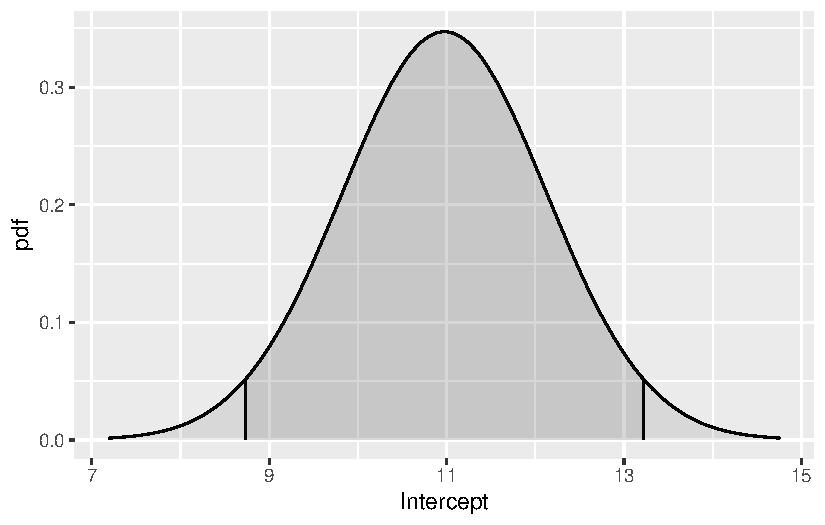
\includegraphics{pedometron_files/figure-pdf/unnamed-chunk-11-1.pdf}

}

\end{figure}

As the credibility interval does not contains 0, we can conclude to a
significant effect of the fixed effect.

We can also plot the posterior distribution of the parameters of the
gaussiant field: range and variance

\begin{Shaded}
\begin{Highlighting}[]
\NormalTok{spde.range.W0 }\OtherTok{\textless{}{-}} \FunctionTok{spde.posterior}\NormalTok{(fit, }\StringTok{"field"}\NormalTok{, }\AttributeTok{what =} \StringTok{"range"}\NormalTok{)}
\NormalTok{spde.logvar.W0 }\OtherTok{\textless{}{-}} \FunctionTok{spde.posterior}\NormalTok{(fit, }\StringTok{"field"}\NormalTok{, }\AttributeTok{what =} \StringTok{"variance"}\NormalTok{)}
\NormalTok{range.plot.W0 }\OtherTok{\textless{}{-}} \FunctionTok{plot}\NormalTok{(spde.range.W0)}
\NormalTok{var.plot.W0 }\OtherTok{\textless{}{-}} \FunctionTok{plot}\NormalTok{(spde.logvar.W0)}
\FunctionTok{multiplot}\NormalTok{(range.plot.W0, var.plot.W0)}
\end{Highlighting}
\end{Shaded}

\begin{figure}[H]

{\centering 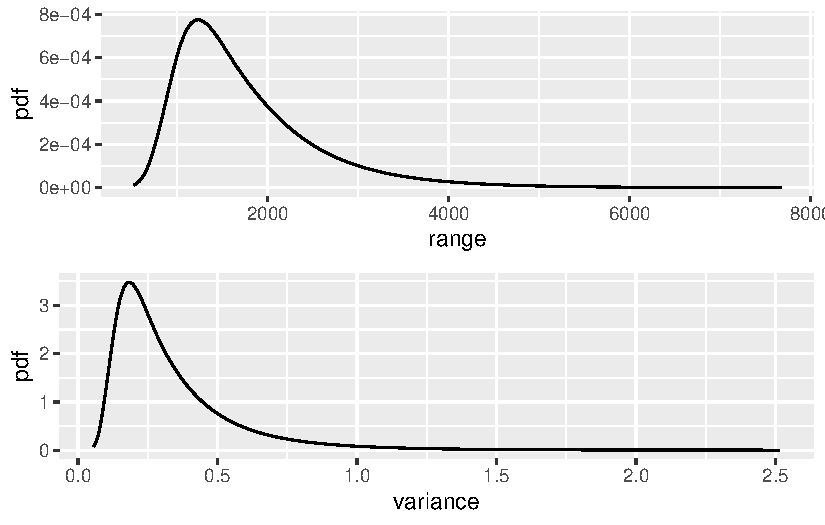
\includegraphics{pedometron_files/figure-pdf/unnamed-chunk-12-1.pdf}

}

\end{figure}

\hypertarget{the-spatial-predictions-with-uncertainty}{%
\subsection{The spatial predictions with
uncertainty}\label{the-spatial-predictions-with-uncertainty}}

We can plot the median, lower 95\% and upper 95\% density surfaces as
follows as follows (assuming that the predicted soil property is in
object \texttt{pred}).

\begin{Shaded}
\begin{Highlighting}[]
\CommentTok{\# correction of negative predictions}
\NormalTok{pred}\SpecialCharTok{$}\NormalTok{q0}\FloatTok{.025}\NormalTok{[pred}\SpecialCharTok{$}\NormalTok{q0}\FloatTok{.025}\SpecialCharTok{\textless{}}\DecValTok{0}\NormalTok{] }\OtherTok{=} \DecValTok{0} 

\FunctionTok{tm\_shape}\NormalTok{(pred) }\SpecialCharTok{+}
  \FunctionTok{tm\_raster}\NormalTok{(}
    \FunctionTok{c}\NormalTok{(}\StringTok{"q0.025"}\NormalTok{,}\StringTok{"median"}\NormalTok{,}\StringTok{"q0.975"}\NormalTok{)}
\NormalTok{    )}
\end{Highlighting}
\end{Shaded}

\begin{figure}[H]

{\centering 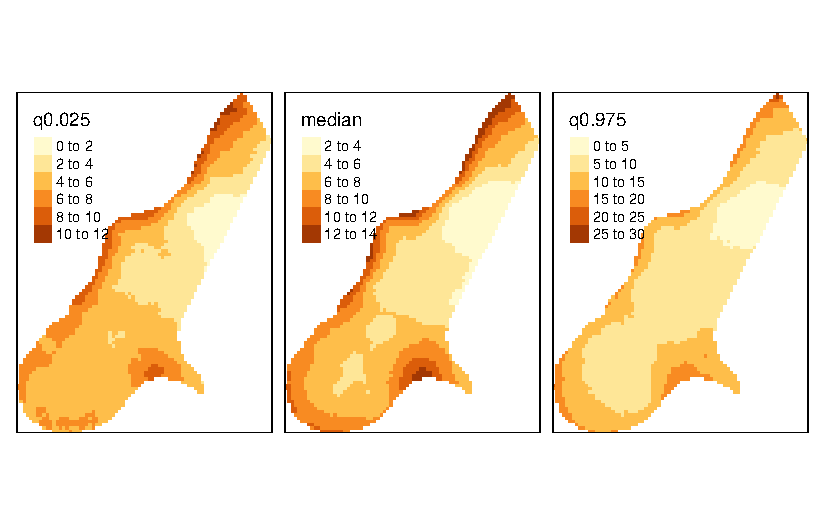
\includegraphics{pedometron_files/figure-pdf/unnamed-chunk-13-1.pdf}

}

\end{figure}

\hypertarget{one-realization-of-the-posterior-distribution}{%
\subsection{One realization of the posterior
distribution}\label{one-realization-of-the-posterior-distribution}}

The sample from the posterior distribution can be mapped as follows.

\begin{Shaded}
\begin{Highlighting}[]
\FunctionTok{tm\_shape}\NormalTok{(pred) }\SpecialCharTok{+} \FunctionTok{tm\_raster}\NormalTok{(}\StringTok{"sample"}\NormalTok{)}
\end{Highlighting}
\end{Shaded}

\begin{figure}[H]

{\centering 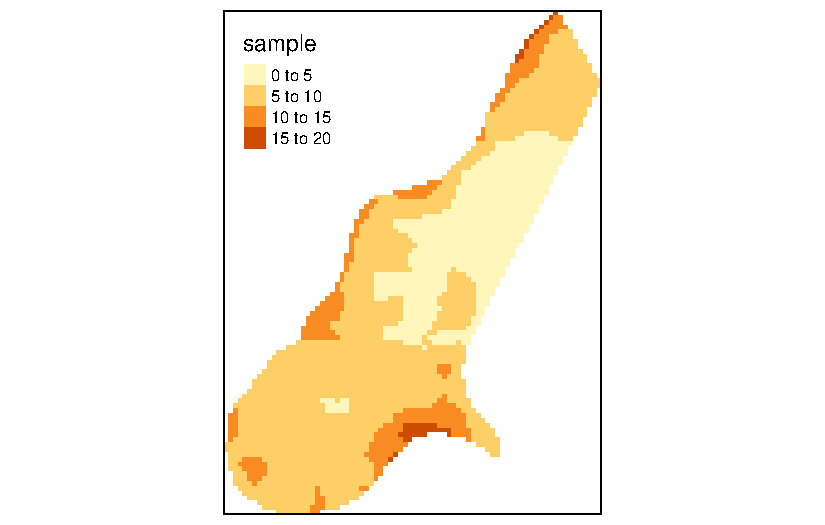
\includegraphics{pedometron_files/figure-pdf/unnamed-chunk-14-1.pdf}

}

\end{figure}

\hypertarget{the-maps-of-the-random-and-the-fixed-effects}{%
\subsection{The maps of the random and the fixed
effects}\label{the-maps-of-the-random-and-the-fixed-effects}}

Next, we plot the 2 effects of the model:

\begin{itemize}
\item
  the spatial Gaussian random field \(W(s)\),
\item
  the fixed effect.
\end{itemize}

\begin{Shaded}
\begin{Highlighting}[]
\NormalTok{pred }\OtherTok{\textless{}{-}} \FunctionTok{predict}\NormalTok{(}
\NormalTok{  fit,}
  \AttributeTok{n.samples =} \DecValTok{100}\NormalTok{,}
\NormalTok{  meuse.grid,}
  \SpecialCharTok{\textasciitilde{}}\NormalTok{ field  ,}
  \AttributeTok{num.threads =} \DecValTok{2}
\NormalTok{)}

\NormalTok{fixed }\OtherTok{\textless{}{-}} \FunctionTok{predict}\NormalTok{(}
\NormalTok{  fit,}
  \AttributeTok{n.samples =} \DecValTok{100}\NormalTok{,}
\NormalTok{  meuse.grid,}
  \SpecialCharTok{\textasciitilde{}}  \FunctionTok{exp}\NormalTok{(Intercept }\SpecialCharTok{+}\NormalTok{ dist)  ,}
  \AttributeTok{num.threads =} \DecValTok{2}
\NormalTok{)}

\NormalTok{pred}\SpecialCharTok{$}\NormalTok{FixedEffect }\OtherTok{\textless{}{-}}\NormalTok{ fixed}\SpecialCharTok{$}\NormalTok{median}
\NormalTok{pred}\SpecialCharTok{$}\NormalTok{W }\OtherTok{\textless{}{-}}\NormalTok{ pred}\SpecialCharTok{$}\NormalTok{median}

\FunctionTok{tm\_shape}\NormalTok{(pred) }\SpecialCharTok{+}
  \FunctionTok{tm\_raster}\NormalTok{(}\FunctionTok{c}\NormalTok{(}\StringTok{"W"}\NormalTok{,}\StringTok{"FixedEffect"}\NormalTok{))}
\end{Highlighting}
\end{Shaded}

\begin{figure}[H]

{\centering 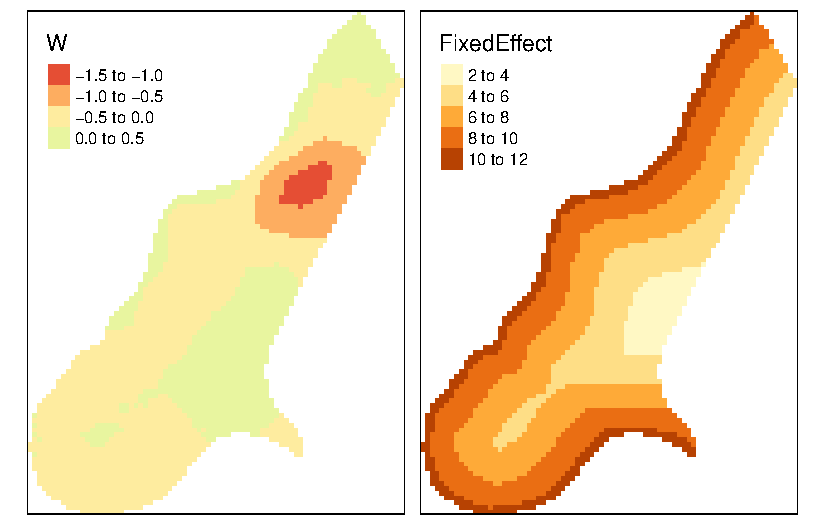
\includegraphics{pedometron_files/figure-pdf/unnamed-chunk-15-1.pdf}

}

\end{figure}

\hypertarget{final-remarks}{%
\section{Final remarks}\label{final-remarks}}

The goal of \href{http://inlabru.org/}{inlabru} is to facilitate spatial
modeling using integrated nested Laplace approximation via the
\href{https://www.r-inla.org/}{R-INLA package}. The recent developments
allow now to construct in a convenient way Bayesian spatial model
(INLA-SPDE) of soil properties and their uncertainty. Model components
are specified with general inputs and mapping methods to the latent
variables, and the predictors are specified via general R expressions.

In their study, Poggio et al. (2016) and Huang et al. (2017) reported
that INLA-SPDE became quite slow when estimating the posterior marginal
distributions of the environmental variables associated with large
datasets. When the number of observations is huge, it is important to
mention that one can improve the performance of the high-dimensional
matrix computations conducted in INLA by using the PARDISO solver
library. It is already full included in the standard INLA installation
but has to be activated through a licence key. To activate it (free for
non commercial uses), go to
https://www.pardiso-project.org/r-inla/\#license to obtain the license,
which will take you at most several minutes. Also, you can type
inla.pardiso() at the R command line for viewing the (very simple)
instructions on how to enable the PARDISO sparse library. Moreover, new
developments are underway for especially data-rich model to achieve even
faster inference, improved numerical stability and scalability using
variational approximation (Van Niekerk et al. 2023).

Heuvelink and Webster (2022) listed a set of challenges for
pedometricians and spatial statisticians to strengthen the role of
spatial statistics. Without being able to solve all of them, it seems to
us that \texttt{INLA} by providing a fully Bayesian modelling in a rapid
and convinent way can provide some answers to some of them, e.g., the
better uncertainty quantification, the change of support, incorporating
attribute and positional measurement uncertainty.

\hypertarget{code-availability}{%
\section{Code availability}\label{code-availability}}

The code is also available on github :
https://github.com/nsaby/pedometron042023

More codes are available here:
https://inlabru-org.github.io/inlabru/articles/web/random\_fields\_2d.html

\hypertarget{references}{%
\section{References}\label{references}}

\hypertarget{refs}{}
\begin{CSLReferences}{1}{0}
\leavevmode\vadjust pre{\hypertarget{ref-HEUVELINK2022100639}{}}%
Heuvelink, Gerard B. M., and Richard Webster. 2022. {``Spatial
Statistics and Soil Mapping: A Blossoming Partnership Under Pressure.''}
\emph{Spatial Statistics} 50: 100639.
https://doi.org/\url{https://doi.org/10.1016/j.spasta.2022.100639}.

\leavevmode\vadjust pre{\hypertarget{ref-Huang2017}{}}%
Huang, Malone, J. 2017. {``{Evaluating a Bayesian modelling approach
(INLA-SPDE) for environmental mapping}.''} \emph{Science of The Total
Environment} 609: 621-\/-632.

\leavevmode\vadjust pre{\hypertarget{ref-Lindgren2011}{}}%
Lindgren, Finn, Håvard Rue, and Johan Lindström. 2011. {``{An explicit
link between Gaussian fields and Gaussian Markov random fields: the
stochastic partial differential equation approach}.''} \emph{Journal of
the Royal Statistical Society: Series B (Statistical Methodology)} 73
(4): 423--98.

\leavevmode\vadjust pre{\hypertarget{ref-Poggio2016}{}}%
Poggio, Laura, Alessandro Gimona, Luigi Spezia, and Mark J Brewer. 2016.
{``{Bayesian spatial modelling of soil properties and their uncertainty:
The example of soil organic matter in Scotland using R-INLA}.''}
\emph{Geoderma} 277: 69--82.

\leavevmode\vadjust pre{\hypertarget{ref-poggio_soilgrids_2021}{}}%
Poggio, L., L. M. de Sousa, N. H. Batjes, G. B. M. Heuvelink, B. Kempen,
E. Ribeiro, and D. Rossiter. 2021. {``{SoilGrids} 2.0: Producing Soil
Information for the Globe with Quantified Spatial Uncertainty.''}
\emph{SOIL} 7 (1): 217--40.
\url{https://doi.org/10.5194/soil-7-217-2021}.

\leavevmode\vadjust pre{\hypertarget{ref-Rue2009}{}}%
Rue, Håvard, Sara Martino, and Nicolas Chopin. 2009. {``{Approximate
Bayesian inference for latent Gaussian models by using integrated nested
Laplace approximations}.''} \emph{Journal of the Royal Statistical
Society: Series b (Statistical Methodology)} 71 (2): 319--92.

\leavevmode\vadjust pre{\hypertarget{ref-VANNIEKERK2023107692}{}}%
Van Niekerk, Janet, Elias Krainski, Denis Rustand, and Håvard Rue. 2023.
{``A New Avenue for Bayesian Inference with INLA.''} \emph{Computational
Statistics \& Data Analysis} 181: 107692.
https://doi.org/\url{https://doi.org/10.1016/j.csda.2023.107692}.

\leavevmode\vadjust pre{\hypertarget{ref-yuan2017point}{}}%
Yuan, Y., F. E. Bachl, F. Lindgren, D. L. Brochers, J. B. Illian, S. T.
Buckland, H. Rue, and T. Gerrodette. 2017. {``Point Process Models for
Spatio-Temporal Distance Sampling Data from a Large-Scale Survey of Blue
Whales.''} \url{https://arxiv.org/abs/1604.06013}.

\end{CSLReferences}



\end{document}
